\documentclass[paper=a4, 11 pt]{report}

\usepackage{color}
\usepackage{hyperref}
\usepackage{graphicx}
\usepackage{cleveref}
\usepackage{multirow}
\hypersetup{
    colorlinks,
    linktoc=all,
    citecolor=black,
    filecolor=black,
    linkcolor=black,
    urlcolor=black
}

\newcommand{\mychapter}[2]{
    \setcounter{chapter}{#1}
    \setcounter{section}{0}
    \chapter*{#2}
    \addcontentsline{toc}{chapter}{#1 #2}
}

\newcommand*{\plogo}{\fbox{$\mathcal{PL}$}} % Generic publisher logo
\newcommand*{\titleGM}{\begingroup % Create the command for including the title page in the document
\hbox{ % Horizontal box
\hspace*{0.2\textwidth} % Whitespace to the left of the title page
\rule{1pt}{\textheight} % Vertical line
\hspace*{0.05\textwidth} % Whitespace between the vertical line and title page text
\parbox[b]{0.75\textwidth}{ % Paragraph box which restricts text to less than the width of the page

{\noindent\Huge\bfseries AttitudeIndicatorMFD \\[0.5\baselineskip] Manual}\\[2\baselineskip] % Title
{\large \textit{\today}}\\[4\baselineskip] % Tagline or further description
{\Large \textsc{Paul Georg Wagner}} % Author name

\vspace{0.5\textheight} % Whitespace between the title block and the publisher
%{\noindent The Publisher \plogo}\\[\baselineskip] % Publisher and logo
}}
\endgroup}


\begin{document}
\titleGM
\pagestyle{empty}
\tableofcontents
\newpage

\mychapter{1}{Introduction}
The AttitudeIndicatorMFD is a MFD plugin that displays an attitude direction indicator (ADI) ball, similar to the navball in Kerbal Space Program.
The ADI ball can show the vessel's current attitude with respect to several reference frames and display velocity and target markers in some of the reference frames.
The two main settings of the MFD are the currently selected mode (text/no-text) and frame of reference (ECL,EQU,OV/OM,LH/LN,NAV).
When in text mode, the MFD shows additional data (altitude, speed, orbital parameters, relative distance/velocity to targets, ...) depending on the currently selected frame of reference, while otherwise only the plain ADI ball is shown.
The different frames of reference are explained more elaborately in the next section.
Depending on the currently selected frame of reference, various markers are shown on the ADI ball, and additional settings are available.

\begin{figure}[h]
	\centering
	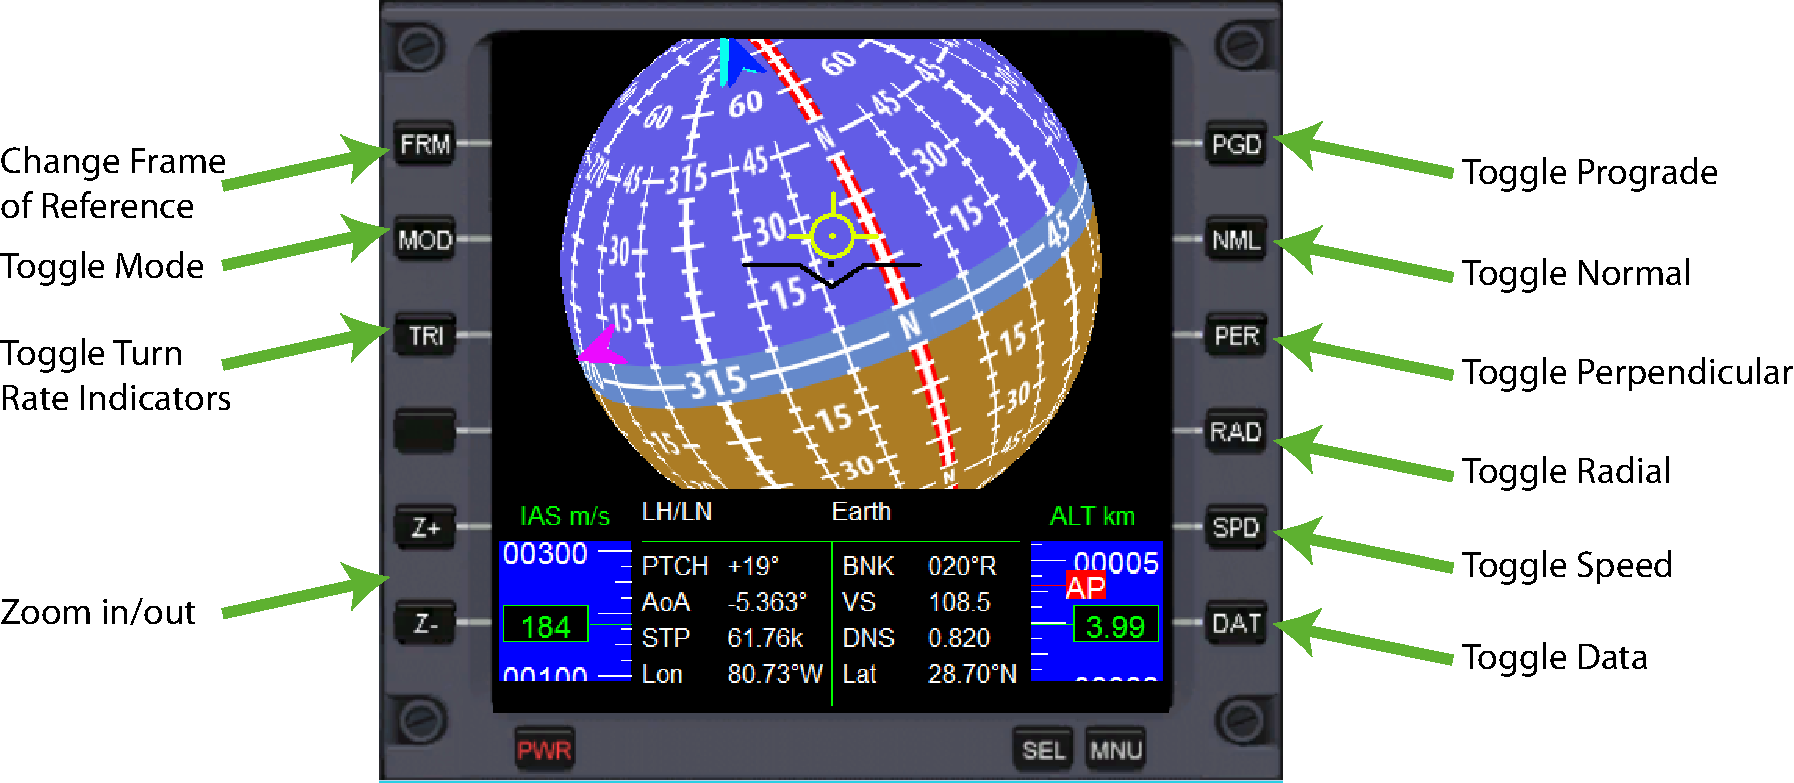
\includegraphics[width=\textwidth]{1_lhln.pdf}
	\caption{Text mode in LH/LN frame}
	\label{fig:overview}
\end{figure}
In \cref{fig:overview} the MFD is shown in text mode in the LH/LN frame.


\mychapter{2}{Reference Frames}
\section{ECL/EQU}
When ECL is selected as frame of reference, the ADI ball shows the current attitude with respect to the ecliptic frame.
When EQU is selected, the frame of reference is the equatorial plane of the currently orbited body.
If the MFD is in text mode, the displayed data is with reference to the current main gravity source acting on the vessel.
In both ECL and EQU mode, no additional markers are available.

\section{OV/OM}
The OV/OM (orbital velocity/orbital momentum) frame of reference rotates the ADI ball to show the current orbit.
In this frame of reference, the ball is aligned to the current orbital plane, with the north mark always facing in the prograde direction.
Additionally, four different pairs of markers are shown on the ball, which ease the orbital orientation.
Those markers are:

\renewcommand{\arraystretch}{2.5}
\begin{center}
\begin{tabular}{ |c  c | c  c| }
  \hline
  Prograde & \includegraphics[scale=.5]{pgd.png} & \includegraphics[scale=.5]{pgd_2.png} & Retrograde \\ \hline
  Normal+ & \includegraphics[scale=.5]{nml.png} & \includegraphics[scale=.5]{nml_2.png} & Normal- \\ \hline
  Perpendicular in & \includegraphics[scale=.5]{perp_in.png} & \includegraphics[scale=.5]{perp_out.png} & Perpendicular out \\ \hline
  Radial in & \includegraphics[scale=.5]{rad_in.png} & \includegraphics[scale=.5]{rad_out.png} & Radial out \\ \hline
\end{tabular}
\end{center}

The markers can be switched off by the buttons on the right side.
In text mode, the reference for the displayed data is always the current main gravity source acting on the vessel.

\section{LH/LN}
The LH/LN (local horizon/local north) frame of reference rotates the ADI ball to display the vessel's current attitude with respect to the planet horizon.
In this mode, the ball shows the same heading as the surface MFD.
As with OV/OM the five marker pairs are shown on the ball, although now with respect to the planet surface instead of the orbital plane.
When in text mode, the ball uses the nearest planetary body as reference for the displayed data.

\section{NAV}
The NAV frame of reference is a special reference frame that depends on the type of signal that is received by the vessel's transmitters.
With the NAV button on the right side, the active transmitter can be selected.
If a signal is received, the ADI ball uses a reference frame relative to that target and shows an additional target marker:

\renewcommand{\arraystretch}{2.7}
\begin{center}
\begin{tabular}{ |c  c | c  c| }
  \hline
  Target & \includegraphics[scale=.5]{tgt.png} & \includegraphics[scale=.5]{tgt_2.png} & Antitarget \\ \hline
\end{tabular}
\end{center}


\subsection{VOR}
When the currently selected transmitter receives a VOR signal, the ADI ball shows the direction of the VOR station using the target marker.
The frame of reference for the ball is the local horizon (LH/LN), so that the ball can be used instead of the surface MFD for navigation.
The only other available marker is a course marker, whose heading can be manually selected using the OB+/OB- switches on the right side.

\renewcommand{\arraystretch}{2.7}
\begin{center}
\begin{tabular}{ |c  c | }
  \hline
  Course Marker & \includegraphics[scale=.5]{crs.png} \\ \hline
\end{tabular}
\end{center}

\subsection{ILS}
When the selected transmitter receives an ILS signal, the ADI ball shows the direction of the target base using the target marker.
Again, the frame of reference for the ball is the local horizon (LH/LN).
The course marker is not changeable when an ILS signal is received and shows the runway heading on the ADI ball.

\begin{figure}[h]
	\centering
	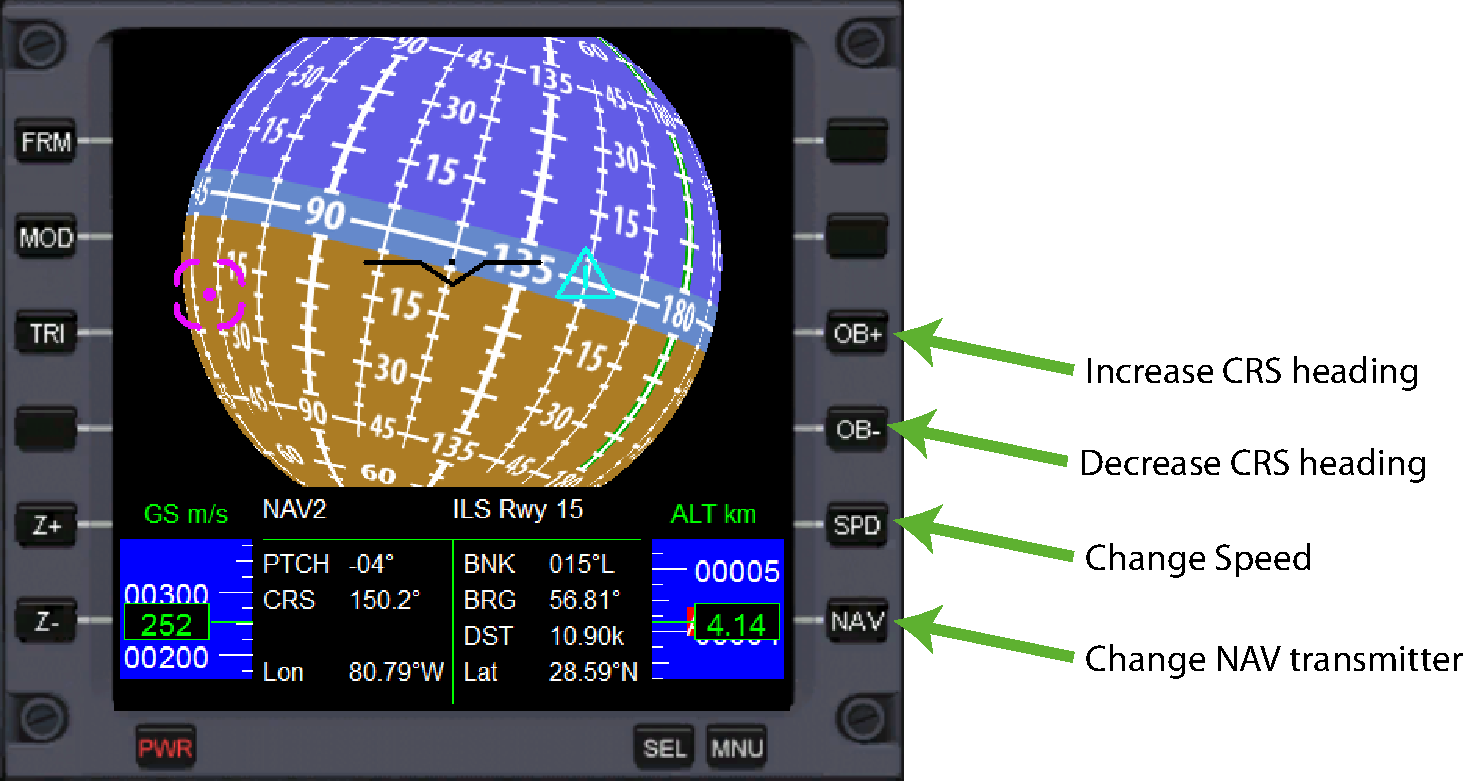
\includegraphics[width=\textwidth]{3_ils.pdf}
	\caption{Text mode in NAV frame with ILS signal}
	\label{fig:ils}
\end{figure}

\subsection{IDS}
When the selected transmitter receives an IDS signal, the ADI ball rotates to a frame relative to the target docking port.
In this frame, the ADI ball's horizon shows the correct rotation angle, so if the vessel is aligned with the horizon, it is correctly rotated relative to the target docking port.
Similarly, the heading indicates the deviation from the correct approach direction to the target docking port.
If the vessel faces north, it is aligned with the target docking port.
Note that when an IDS signal is received, the ball can be switched between two different frames of reference using the REF button on the right side.
In the VESSEL frame, the ball shows the current relative attitude with respect to the vessel's center, while in DOCKPORT frame, the ball uses a coordinate system centered at vessel's docking port.
This is especially handy if the docking port is not aligned with the vessel's nose (like in the Space Shuttle).

In both frames the target marker shows the direction to the target docking port, while the prograde/retrograde markers show the current velocity vector relative to the target.
To ease the docking process, when in text mode the ball shows additional information about the relative distance and velocity.
Also approach indicators, similar to the ones in the docking MFD, are displayed.

\begin{figure}[h]
	\centering
	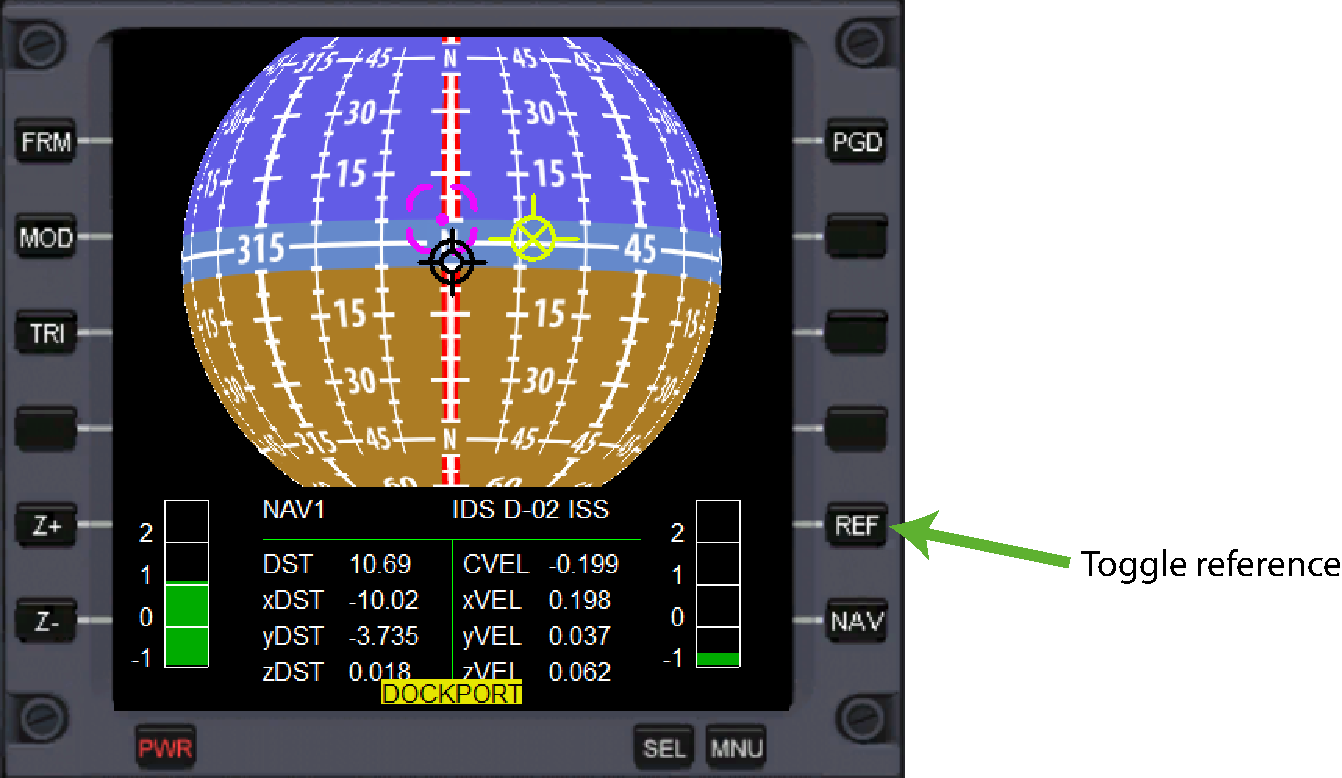
\includegraphics[width=\textwidth]{4_ids_2.pdf}
	\caption{Text mode in NAV frame with IDS signal}
	\label{fig:ids}
\end{figure}

\subsection{XPDR}
An XPDR signal is handled similarly to an IDS signal, only that the used reference frame is always the current vessel's coordinate system.

\subsection{VTOL}
When the selected transmitter receives a VTOL signal, the ball once again shows the current local heading with respect to the planet surface (as in VOR and ILS mode).
The target marker shows the direction to the landing pad, while the prograde/retrograde marker shows the current velocity vector relative to the surface.
As with IDS signals, one can change the current frame of reference using the REF button on the right side.
In VESSEL frame the attitude is shown with reference to the vessel's nose, while in TOP frame, the view is pitched 90 degrees down towards the ground.
This reference frame eases the final landing approach, as the target marker is usually directly below the vessel.
Again, in text mode the ball shows additional navigation information, along with approach indicators similar to the ones from the VTOL MFD.

\mychapter{3}{Configuration}
The AttitudeIndicatorMFD can be configured using the configuration file stored in /Config/MFD/AttitudeIndicatorMFD.cfg.

\section{Texture}
The texture that is used for the ADI ball can be replaced by changing the \texttt{texture} entry in the configuration file.
The entry should contain a path to a bitmap file relative to the Orbiter main directory.
The bitmap should have a resolution of 1024x512 pixels.

\section{Colors}
The colors for some indicators and the markers can be changed in the configuration file.
This way other textures can be easily accomodated with fitting marker colors.
The colors are specified in RGB by using one configuration value of range 0-255 per color.

\renewcommand{\arraystretch}{1}
\begin{center}
\begin{tabular}{ |l  l  l| }
  \hline
  \textbf{Keys} & \textbf{Default} & \textbf{Description} \\ \hline
   progradeR & 221 & \multirow{3}{*}{Prograde/Retrograde Marker Color} \\
   progradeG & 255 &  \\
   progradeB & 0 &  \\ \hline
   normalR & 235 & \multirow{3}{*}{Normal/Antinormal Marker Color} \\
   normalG & 11 &  \\
   normalB & 255 &  \\ \hline
   perpendicularR & 9 & \multirow{3}{*}{Perpendicular in/out Marker Color} \\
   perpendicularG & 254 &  \\
   perpendicularB & 239 &  \\ \hline
   radialR & 0 & \multirow{3}{*}{Radial in/out Marker Color} \\
   radialG & 34 &  \\
   radialB & 255 &  \\ \hline
   targetR & 235 & \multirow{3}{*}{Target Marker Color} \\
   targetG & 11 &  \\
   targetB & 255 &  \\ \hline
   wingR & 0 & \multirow{3}{*}{Wing/Dockingport Color} \\
   wingG & 0 &  \\
   wingB & 0 &  \\ \hline
   indicatorR & 255 & \multirow{3}{*}{Turn Rate Indicator Color} \\
   indicatorG & 255 &  \\
   indicatorB & 255 &  \\ \hline
   turnVectorR & 0 & \multirow{3}{*}{Turn Vector Indicator Color} \\
   turnVectorG & 255 &  \\
   turnVectorB & 0 &  \\ \hline
\end{tabular}
\end{center}

\section{Default Settings}
Some configuration values can be used to determine the default settings to be used by the ADI ball when a new instance is created.
\begin{center}
\begin{tabular}{ |l  l  l| }
  \hline
  \textbf{Keys} & \textbf{Default} & \textbf{Description} \\ \hline
   startPrograde & TRUE & Start with prograde/retrograde marker enabled \\ \hline
   startNormal & TRUE & Start with normal/antinormal marker enabled \\ \hline
   startPerpendicular & TRUE & Start with perpendicular in/out marker enabled \\ \hline
   startRadial & TRUE & Start with radial in/out marker enabled \\ \hline
   \multirow{2}{*}{startTurnVectorMode} & \multirow{2}{*}{0} & Start with turn rate indicators disabled(0),\\
    &  & as bar indicators (1) or overlay turn vector (2) \\ \hline
   \multirow{2}{*}{startMode} & \multirow{2}{*}{0} & Start in text mode(0),\\
    &  & Start in no-text mode(1) \\ \hline
   \multirow{2}{*}{startFrame} & \multirow{2}{*}{0} & Start in ECL(0), in EQU(1)\\
    &  & in OV/OM(2), in LH/LN(3) or in NAV(4), \\ \hline
\end{tabular}
\end{center}

\mychapter{4}{Abbreviations}
The following abbreviations are used for the displayed parameters in text mode.

\begin{center}
\begin{tabular}{ |l  l  l| }
  \hline
  \textbf{Short} & \textbf{Long} & \textbf{Frame} \\ \hline
   ApA & Apoapsis height from surface (m) & ECL,EQU,OV/OM,LH/LN \\ \hline
   PeA & Periapsis height from surface (m) & ECL,EQU,OV/OM,LH/LN \\ \hline
   ApT & Time to apoapsis (s) & ECL,EQU,OV/OM,LH/LN \\ \hline
   PeT & Time to periapsis (s) & ECL,EQU,OV/OM,LH/LN \\ \hline
   Ecc & Eccentricity & ECL,EQU,OV/OM,LH/LN \\ \hline
   Inc & Inclination (deg) & ECL,EQU,OV/OM,LH/LN \\ \hline
   LAN & Longitude of ascending node (deg) & ECL,EQU,OV/OM,LH/LN \\ \hline
   T & Orbital period (s) & ECL,EQU,OV/OM,LH/LN \\ \hline
   PTCH & Pitch (deg) & LH/LN,VOR,ILS,VTOL \\ \hline
   BNK & Bank (deg) & LH/LN,VOR,ILS,VTOL \\ \hline
   AoA & Angle of attack (deg) & LH/LN \\ \hline
   VS & Vertical speed ($\frac{m}{s}$) & LH/LN \\ \hline
   STP & Static pressure (Pa) & LH/LN \\ \hline
   DNS & Density ($\frac{kg}{m^3}$) & LH/LN \\ \hline
   Lon & Longitude (deg) & LH/LN,VOR,ILS \\ \hline
   Lat & Latitude (deg) & LH/LN,VOR,ILS \\ \hline
   CRS & Course marker (deg) & VOR,ILS \\ \hline
   BRG & Bearing (deg) & VOR,ILS \\ \hline
   DST & Distance (m) & VOR,ILS,XPDR,VTOL \\ \hline
   CVEL & Closing velocity ($\frac{m}{s}$) & IDS,XPDR \\ \hline
   ALT & Altitude (m) & VTOL \\ \hline
   VSPD & Vertical speed ($\frac{m}{s}$) & VTOL \\ \hline
   HSPD & Horizontal speed ($\frac{m}{s}$) & VTOL \\ \hline
   HDG & Heading (deg) & VTOL \\ \hline
   DIR & Direction of base (deg) & VTOL \\ \hline
\end{tabular}
\end{center}

%\bibliography{}

\end{document}